% Options for packages loaded elsewhere
\PassOptionsToPackage{unicode}{hyperref}
\PassOptionsToPackage{hyphens}{url}
\PassOptionsToPackage{dvipsnames,svgnames,x11names}{xcolor}
%
\documentclass[
  10pt,
  ignorenonframetext,
  aspectratio=169]{beamer}
\usepackage{pgfpages}
\setbeamertemplate{caption}[numbered]
\setbeamertemplate{caption label separator}{: }
\setbeamercolor{caption name}{fg=normal text.fg}
\beamertemplatenavigationsymbolsempty
% Prevent slide breaks in the middle of a paragraph
\widowpenalties 1 10000
\raggedbottom
\setbeamertemplate{part page}{
  \centering
  \begin{beamercolorbox}[sep=16pt,center]{part title}
    \usebeamerfont{part title}\insertpart\par
  \end{beamercolorbox}
}
\setbeamertemplate{section page}{
  \centering
  \begin{beamercolorbox}[sep=12pt,center]{part title}
    \usebeamerfont{section title}\insertsection\par
  \end{beamercolorbox}
}
\setbeamertemplate{subsection page}{
  \centering
  \begin{beamercolorbox}[sep=8pt,center]{part title}
    \usebeamerfont{subsection title}\insertsubsection\par
  \end{beamercolorbox}
}
\AtBeginPart{
  \frame{\partpage}
}
\AtBeginSection{
  \ifbibliography
  \else
    \frame{\sectionpage}
  \fi
}
\AtBeginSubsection{
  \frame{\subsectionpage}
}
\usepackage{amsmath,amssymb}
\usepackage{iftex}
\ifPDFTeX
  \usepackage[T1]{fontenc}
  \usepackage[utf8]{inputenc}
  \usepackage{textcomp} % provide euro and other symbols
\else % if luatex or xetex
  \usepackage{unicode-math} % this also loads fontspec
  \defaultfontfeatures{Scale=MatchLowercase}
  \defaultfontfeatures[\rmfamily]{Ligatures=TeX,Scale=1}
\fi
\usepackage{lmodern}
\usetheme[]{Singapore}
\ifPDFTeX\else
  % xetex/luatex font selection
\fi
% Use upquote if available, for straight quotes in verbatim environments
\IfFileExists{upquote.sty}{\usepackage{upquote}}{}
\IfFileExists{microtype.sty}{% use microtype if available
  \usepackage[]{microtype}
  \UseMicrotypeSet[protrusion]{basicmath} % disable protrusion for tt fonts
}{}
\makeatletter
\@ifundefined{KOMAClassName}{% if non-KOMA class
  \IfFileExists{parskip.sty}{%
    \usepackage{parskip}
  }{% else
    \setlength{\parindent}{0pt}
    \setlength{\parskip}{6pt plus 2pt minus 1pt}}
}{% if KOMA class
  \KOMAoptions{parskip=half}}
\makeatother
\usepackage{xcolor}
\newif\ifbibliography
\usepackage{color}
\usepackage{fancyvrb}
\newcommand{\VerbBar}{|}
\newcommand{\VERB}{\Verb[commandchars=\\\{\}]}
\DefineVerbatimEnvironment{Highlighting}{Verbatim}{commandchars=\\\{\}}
% Add ',fontsize=\small' for more characters per line
\usepackage{framed}
\definecolor{shadecolor}{RGB}{48,48,48}
\newenvironment{Shaded}{\begin{snugshade}}{\end{snugshade}}
\newcommand{\AlertTok}[1]{\textcolor[rgb]{1.00,0.81,0.69}{#1}}
\newcommand{\AnnotationTok}[1]{\textcolor[rgb]{0.50,0.62,0.50}{\textbf{#1}}}
\newcommand{\AttributeTok}[1]{\textcolor[rgb]{0.80,0.80,0.80}{#1}}
\newcommand{\BaseNTok}[1]{\textcolor[rgb]{0.86,0.64,0.64}{#1}}
\newcommand{\BuiltInTok}[1]{\textcolor[rgb]{0.80,0.80,0.80}{#1}}
\newcommand{\CharTok}[1]{\textcolor[rgb]{0.86,0.64,0.64}{#1}}
\newcommand{\CommentTok}[1]{\textcolor[rgb]{0.50,0.62,0.50}{#1}}
\newcommand{\CommentVarTok}[1]{\textcolor[rgb]{0.50,0.62,0.50}{\textbf{#1}}}
\newcommand{\ConstantTok}[1]{\textcolor[rgb]{0.86,0.64,0.64}{\textbf{#1}}}
\newcommand{\ControlFlowTok}[1]{\textcolor[rgb]{0.94,0.87,0.69}{#1}}
\newcommand{\DataTypeTok}[1]{\textcolor[rgb]{0.87,0.87,0.75}{#1}}
\newcommand{\DecValTok}[1]{\textcolor[rgb]{0.86,0.86,0.80}{#1}}
\newcommand{\DocumentationTok}[1]{\textcolor[rgb]{0.50,0.62,0.50}{#1}}
\newcommand{\ErrorTok}[1]{\textcolor[rgb]{0.76,0.75,0.62}{#1}}
\newcommand{\ExtensionTok}[1]{\textcolor[rgb]{0.80,0.80,0.80}{#1}}
\newcommand{\FloatTok}[1]{\textcolor[rgb]{0.75,0.75,0.82}{#1}}
\newcommand{\FunctionTok}[1]{\textcolor[rgb]{0.94,0.94,0.56}{#1}}
\newcommand{\ImportTok}[1]{\textcolor[rgb]{0.80,0.80,0.80}{#1}}
\newcommand{\InformationTok}[1]{\textcolor[rgb]{0.50,0.62,0.50}{\textbf{#1}}}
\newcommand{\KeywordTok}[1]{\textcolor[rgb]{0.94,0.87,0.69}{#1}}
\newcommand{\NormalTok}[1]{\textcolor[rgb]{0.80,0.80,0.80}{#1}}
\newcommand{\OperatorTok}[1]{\textcolor[rgb]{0.94,0.94,0.82}{#1}}
\newcommand{\OtherTok}[1]{\textcolor[rgb]{0.94,0.94,0.56}{#1}}
\newcommand{\PreprocessorTok}[1]{\textcolor[rgb]{1.00,0.81,0.69}{\textbf{#1}}}
\newcommand{\RegionMarkerTok}[1]{\textcolor[rgb]{0.80,0.80,0.80}{#1}}
\newcommand{\SpecialCharTok}[1]{\textcolor[rgb]{0.86,0.64,0.64}{#1}}
\newcommand{\SpecialStringTok}[1]{\textcolor[rgb]{0.80,0.58,0.58}{#1}}
\newcommand{\StringTok}[1]{\textcolor[rgb]{0.80,0.58,0.58}{#1}}
\newcommand{\VariableTok}[1]{\textcolor[rgb]{0.80,0.80,0.80}{#1}}
\newcommand{\VerbatimStringTok}[1]{\textcolor[rgb]{0.80,0.58,0.58}{#1}}
\newcommand{\WarningTok}[1]{\textcolor[rgb]{0.50,0.62,0.50}{\textbf{#1}}}
\setlength{\emergencystretch}{3em} % prevent overfull lines
\providecommand{\tightlist}{%
  \setlength{\itemsep}{0pt}\setlength{\parskip}{0pt}}
\setcounter{secnumdepth}{-\maxdimen} % remove section numbering
\newenvironment{cols}[1][]{}{}

\newenvironment{col}[1]{\begin{minipage}{#1}\ignorespaces}{%
\end{minipage}
\ifhmode\unskip\fi
\aftergroup\useignorespacesandallpars}

\def\useignorespacesandallpars#1\ignorespaces\fi{%
#1\fi\ignorespacesandallpars}

\makeatletter
\def\ignorespacesandallpars{%
  \@ifnextchar\par
    {\expandafter\ignorespacesandallpars\@gobble}%
    {}%
}
\makeatother
\ifLuaTeX
  \usepackage{selnolig}  % disable illegal ligatures
\fi
\usepackage[]{natbib}
\bibliographystyle{plainnat}
\IfFileExists{bookmark.sty}{\usepackage{bookmark}}{\usepackage{hyperref}}
\IfFileExists{xurl.sty}{\usepackage{xurl}}{} % add URL line breaks if available
\urlstyle{same}
\hypersetup{
  pdftitle={Sentiment Analysis},
  pdfauthor={Max Callaghan},
  colorlinks=true,
  linkcolor={Maroon},
  filecolor={Maroon},
  citecolor={Blue},
  urlcolor={blue},
  pdfcreator={LaTeX via pandoc}}

\title{Sentiment Analysis}
\author{Max Callaghan}
\date{2023-11-13}

\begin{document}
\frame{\titlepage}

\hypertarget{introduction-and-objectives}{%
\section{Introduction and
Objectives}\label{introduction-and-objectives}}

\begin{frame}{Assignment 4}
\protect\hypertarget{assignment-4}{}
Assignment 4 is still live. If you have issues, or encounter
difficulties, raise an issue on the Github repository, or write me an
email!
\end{frame}

\begin{frame}{Assignment 5}
\protect\hypertarget{assignment-5}{}
Assignment 5 is approaching, and you should have a clear idea of what
you want to do by the end of next week.

Feel free to ask for quick feedback on any ideas you have in the coming
days
\end{frame}

\begin{frame}{Objectives}
\protect\hypertarget{objectives}{}
By now we have spent a long time understanding how to \textbf{represent}
texts in simple and more complex ways.

We've also started asking questions about texts: What are they about?

Today we will ask a new question about texts: what sentiment does it
express?
\end{frame}

\hypertarget{intro-to-sentiment-analysis}{%
\section{Intro to sentiment
analysis}\label{intro-to-sentiment-analysis}}

\begin{frame}{What is a sentiment?}
\protect\hypertarget{what-is-a-sentiment}{}
The emotion embodied in a text. Often reduced to positive-negative, but
can encompass a more complex range of emotions like joy, sadness, anger.
\end{frame}

\begin{frame}{Sentiment analysis as classification}
\protect\hypertarget{sentiment-analysis-as-classification}{}
In some ways, sentiment analysis is a special case of the broader
\textbf{classification} task, where we ask:

\begin{itemize}
\tightlist
\item
  Is a text of class A or not? or,
\item
  Is a text of class A or B
\end{itemize}

With sentiment analysis, the classes are inherent features of how humans
use language which \emph{generalise} (to a certain extent) across
contexts.
\end{frame}

\begin{frame}{An overview of techniques to do sentiment analysis}
\protect\hypertarget{an-overview-of-techniques-to-do-sentiment-analysis}{}
Doing sentiment analysis usually involves \textbf{rule-based} or
\textbf{statistical machine-learning} techniques

\begin{itemize}
  \item<2->Assessing sentiment based on counting words have a predefined sentiment
  \item<3->Using a classifier that has been trained to identify sentiment with text examples that have been labelled.
\end{itemize}
\end{frame}

\hypertarget{lexicon-based-sentiment-analysis}{%
\section{Lexicon-based sentiment
analysis}\label{lexicon-based-sentiment-analysis}}

\begin{frame}[fragile]{Positive and negative words}
\protect\hypertarget{positive-and-negative-words}{}
We know about the ``bag of words'' model of representing texts.

We also know that some words are rather positive, whereas some are
rather negative.

Consider the texts:

\medskip

\begin{Shaded}
\begin{Highlighting}[]
\NormalTok{texts }\OtherTok{\textless{}{-}} \FunctionTok{c}\NormalTok{(}
  \StringTok{"Elon Musk is a champion of free speech"}\NormalTok{,}
  \StringTok{"It\textquotesingle{}s a terrible shame to see mashed potato thrown at art"}
\NormalTok{)}
\end{Highlighting}
\end{Shaded}

\medskip

Do they express positive or negative sentiment? How can we tell?
\end{frame}

\begin{frame}[fragile]{Using Lexicons in R}
\protect\hypertarget{using-lexicons-in-r}{}
We can import a lexicon in R using tidytext. Each row, contains a word
and its value

\medskip

\begin{Shaded}
\begin{Highlighting}[]
\FunctionTok{library}\NormalTok{(tidytext)}
\FunctionTok{library}\NormalTok{(dplyr)}
\NormalTok{lex }\OtherTok{\textless{}{-}} \FunctionTok{get\_sentiments}\NormalTok{(}\StringTok{"afinn"}\NormalTok{)}
\FunctionTok{sample\_n}\NormalTok{(lex, }\DecValTok{5}\NormalTok{)}
\end{Highlighting}
\end{Shaded}

\begin{verbatim}
## # A tibble: 5 x 2
##   word      value
##   <chr>     <dbl>
## 1 allow         1
## 2 welcomed      2
## 3 triumph       4
## 4 cynic        -2
## 5 abilities     2
\end{verbatim}
\end{frame}

\begin{frame}[fragile]{Using Lexicons in R}
\protect\hypertarget{using-lexicons-in-r-1}{}
Note that the Afinn lexicon is not the newest version. We can just read
this in directly from the author's Github page.

\medskip

\begin{Shaded}
\begin{Highlighting}[]
\FunctionTok{library}\NormalTok{(readr)}
\NormalTok{lex }\OtherTok{\textless{}{-}} \FunctionTok{read\_tsv}\NormalTok{(}
  \StringTok{"https://raw.githubusercontent.com/fnielsen/afinn/master/afinn/data/AFINN{-}en{-}165.txt"}\NormalTok{,}
  \AttributeTok{col\_names=}\FunctionTok{c}\NormalTok{(}\StringTok{"word"}\NormalTok{,}\StringTok{"value"}\NormalTok{)}
\NormalTok{)}

\NormalTok{lex}
\end{Highlighting}
\end{Shaded}

\begin{verbatim}
## # A tibble: 3,382 x 2
##    word       value
##    <chr>      <dbl>
##  1 abandon       -2
##  2 abandoned     -2
##  3 abandons      -2
##  4 abducted      -2
##  5 abduction     -2
##  6 abductions    -2
##  7 abhor         -3
##  8 abhorred      -3
##  9 abhorrent     -3
## 10 abhors        -3
## # ... with 3,372 more rows
\end{verbatim}
\end{frame}

\begin{frame}[fragile]{Using Lexicons in R}
\protect\hypertarget{using-lexicons-in-r-2}{}
There are a few different lexicons, compiled by different authors, using
different techniques involving amazon turk and author knowledge, which
encode different types of emotions.

\medskip

\begin{Shaded}
\begin{Highlighting}[]
\FunctionTok{library}\NormalTok{(tidytext)}
\FunctionTok{library}\NormalTok{(dplyr)}
\NormalTok{lex }\OtherTok{\textless{}{-}} \FunctionTok{get\_sentiments}\NormalTok{(}\StringTok{"nrc"}\NormalTok{)}
\FunctionTok{head}\NormalTok{(lex)}
\end{Highlighting}
\end{Shaded}

\begin{verbatim}
## # A tibble: 6 x 2
##   word      sentiment
##   <chr>     <chr>    
## 1 abacus    trust    
## 2 abandon   fear     
## 3 abandon   negative 
## 4 abandon   sadness  
## 5 abandoned anger    
## 6 abandoned fear
\end{verbatim}
\end{frame}

\begin{frame}[fragile]{Using Lexicons in R}
\protect\hypertarget{using-lexicons-in-r-3}{}
We can also put our usual document feature matrix into a similar format

\medskip
\scriptsize

\begin{Shaded}
\begin{Highlighting}[]
\FunctionTok{library}\NormalTok{(quanteda)}
\NormalTok{dfmat }\OtherTok{\textless{}{-}}\NormalTok{ texts }\SpecialCharTok{\%\textgreater{}\%}
\NormalTok{  tokens }\SpecialCharTok{\%\textgreater{}\%}
  \FunctionTok{dfm}\NormalTok{()}

\NormalTok{text\_tokens }\OtherTok{\textless{}{-}} \FunctionTok{tidy}\NormalTok{(dfmat)}
\FunctionTok{head}\NormalTok{(text\_tokens)}
\end{Highlighting}
\end{Shaded}

\begin{verbatim}
## # A tibble: 6 x 3
##   document term     count
##   <chr>    <chr>    <dbl>
## 1 text1    elon         1
## 2 text1    musk         1
## 3 text1    is           1
## 4 text1    a            1
## 5 text2    a            1
## 6 text1    champion     1
\end{verbatim}
\end{frame}

\begin{frame}[fragile]{Tidy lexicons}
\protect\hypertarget{tidy-lexicons}{}
Now we can join these to see which words in the texts have what
sentiment

\medskip
\scriptsize

\begin{Shaded}
\begin{Highlighting}[]
\NormalTok{lex }\OtherTok{\textless{}{-}} \FunctionTok{read\_tsv}\NormalTok{(}\StringTok{"https://raw.githubusercontent.com/fnielsen/afinn/master/afinn/data/AFINN{-}en{-}165.txt"}\NormalTok{, }\AttributeTok{col\_names=}\FunctionTok{c}\NormalTok{(}\StringTok{"word"}\NormalTok{,}\StringTok{"value"}\NormalTok{))}
\NormalTok{dfmat }\OtherTok{\textless{}{-}}\NormalTok{ texts }\SpecialCharTok{\%\textgreater{}\%}
\NormalTok{  tokens }\SpecialCharTok{\%\textgreater{}\%}
  \FunctionTok{dfm}\NormalTok{()}

\NormalTok{text\_tokens }\OtherTok{\textless{}{-}} \FunctionTok{tidy}\NormalTok{(dfmat) }\SpecialCharTok{\%\textgreater{}\%} 
  \FunctionTok{inner\_join}\NormalTok{(lex, }\AttributeTok{by=}\FunctionTok{c}\NormalTok{(}\StringTok{"term"} \OtherTok{=} \StringTok{"word"}\NormalTok{))}

\NormalTok{text\_tokens}
\end{Highlighting}
\end{Shaded}

\begin{verbatim}
## # A tibble: 4 x 4
##   document term     count value
##   <chr>    <chr>    <dbl> <dbl>
## 1 text1    champion     1     2
## 2 text1    free         1     1
## 3 text2    terrible     1    -3
## 4 text2    shame        1    -2
\end{verbatim}
\end{frame}

\begin{frame}[fragile]{Tidy lexicons}
\protect\hypertarget{tidy-lexicons-1}{}
We can then just sum word scores for each document to get a sentiment
score for that document

\medskip
\scriptsize

\begin{Shaded}
\begin{Highlighting}[]
\NormalTok{doc\_sentiments }\OtherTok{\textless{}{-}} \FunctionTok{tidy}\NormalTok{(dfmat) }\SpecialCharTok{\%\textgreater{}\%} 
  \FunctionTok{inner\_join}\NormalTok{(lex, }\AttributeTok{by=}\FunctionTok{c}\NormalTok{(}\StringTok{"term"} \OtherTok{=} \StringTok{"word"}\NormalTok{)) }\SpecialCharTok{\%\textgreater{}\%}
  \FunctionTok{mutate}\NormalTok{(}\AttributeTok{value=}\NormalTok{value}\SpecialCharTok{*}\NormalTok{count) }\SpecialCharTok{\%\textgreater{}\%}
  \FunctionTok{group\_by}\NormalTok{(document) }\SpecialCharTok{\%\textgreater{}\%}
  \FunctionTok{summarise}\NormalTok{(}\AttributeTok{value =} \FunctionTok{sum}\NormalTok{(value))}

\NormalTok{doc\_sentiments}
\end{Highlighting}
\end{Shaded}

\begin{verbatim}
## # A tibble: 2 x 2
##   document value
##   <chr>    <dbl>
## 1 text1        3
## 2 text2       -5
\end{verbatim}
\end{frame}

\begin{frame}[fragile]{Using Lexicons in Python}
\protect\hypertarget{using-lexicons-in-python}{}
Doing this in Python is very similar. We can use the afinn package to
access the afinn lexion

\medskip
\scriptsize

\begin{Shaded}
\begin{Highlighting}[]
\ImportTok{import}\NormalTok{ pandas }\ImportTok{as}\NormalTok{ pd}
\ImportTok{from}\NormalTok{ sklearn.feature\_extraction.text }\ImportTok{import}\NormalTok{ CountVectorizer}
\ImportTok{from}\NormalTok{ afinn }\ImportTok{import}\NormalTok{ Afinn}
\ImportTok{import}\NormalTok{ numpy }\ImportTok{as}\NormalTok{ np}

\NormalTok{afinn }\OperatorTok{=}\NormalTok{ Afinn()}
\NormalTok{lex }\OperatorTok{=}\NormalTok{ pd.DataFrame(afinn.\_dict.items(),columns}\OperatorTok{=}\NormalTok{[}\StringTok{"word"}\NormalTok{,}\StringTok{"value"}\NormalTok{])}

\NormalTok{lex.head()}
\end{Highlighting}
\end{Shaded}

\begin{verbatim}
##         word  value
## 0    abandon     -2
## 1  abandoned     -2
## 2   abandons     -2
## 3   abducted     -2
## 4  abduction     -2
\end{verbatim}
\end{frame}

\begin{frame}[fragile]{Using Lexicons in Python}
\protect\hypertarget{using-lexicons-in-python-1}{}
Then, in the same way, we can put our dfm into a ``tidy'' form and merge
with our lexicon

\medskip
\scriptsize

\begin{Shaded}
\begin{Highlighting}[]
\NormalTok{texts }\OperatorTok{=}\NormalTok{ [}
    \StringTok{"Elon Musk is a champion of free speech"}\NormalTok{,}
    \StringTok{"It\textquotesingle{}s a terrible shame to see mashed potato thrown at art"}
\NormalTok{]}
\NormalTok{vec }\OperatorTok{=}\NormalTok{ CountVectorizer()}
\NormalTok{dfmat }\OperatorTok{=}\NormalTok{ vec.fit\_transform(texts)}

\KeywordTok{def}\NormalTok{ tidy\_dfmat(dfmat, vec):}
\NormalTok{    nz }\OperatorTok{=}\NormalTok{ dfmat.nonzero()}
\NormalTok{    text\_df }\OperatorTok{=}\NormalTok{ pd.DataFrame(\{}
        \StringTok{"document"}\NormalTok{: np.array(texts)[nz[}\DecValTok{0}\NormalTok{]],}
        \StringTok{"term"}\NormalTok{: vec.get\_feature\_names\_out()[nz[}\DecValTok{1}\NormalTok{]],}
        \StringTok{"count"}\NormalTok{: dfmat[nz].A1}
\NormalTok{    \})}
    \ControlFlowTok{return}\NormalTok{ text\_df}
\NormalTok{text\_df }\OperatorTok{=}\NormalTok{ tidy\_dfmat(dfmat, vec)}
\NormalTok{text\_tokens }\OperatorTok{=}\NormalTok{ text\_df.merge(lex, left\_on}\OperatorTok{=}\StringTok{"term"}\NormalTok{, right\_on}\OperatorTok{=}\StringTok{"word"}\NormalTok{)}
\NormalTok{text\_tokens[}\StringTok{"value"}\NormalTok{] }\OperatorTok{*=}\NormalTok{ text\_tokens[}\StringTok{"count"}\NormalTok{]}
\NormalTok{text\_tokens}
\end{Highlighting}
\end{Shaded}

\begin{verbatim}
##                                             document      term  ...      word value
## 0             Elon Musk is a champion of free speech  champion  ...  champion     2
## 1             Elon Musk is a champion of free speech      free  ...      free     1
## 2  It's a terrible shame to see mashed potato thr...  terrible  ...  terrible    -3
## 3  It's a terrible shame to see mashed potato thr...     shame  ...     shame    -2
## 
## [4 rows x 5 columns]
\end{verbatim}
\end{frame}

\begin{frame}[fragile]{Using Lexicons in Python}
\protect\hypertarget{using-lexicons-in-python-2}{}
In the very same way, we can sum across documents \medskip \scriptsize

\begin{Shaded}
\begin{Highlighting}[]
\NormalTok{doc\_sentiments }\OperatorTok{=}\NormalTok{ text\_tokens.groupby(}\StringTok{"document"}\NormalTok{)[}\StringTok{"value"}\NormalTok{].}\BuiltInTok{sum}\NormalTok{()}
\NormalTok{doc\_sentiments}
\end{Highlighting}
\end{Shaded}

\begin{verbatim}
## document
## Elon Musk is a champion of free speech                      3
## It's a terrible shame to see mashed potato thrown at art   -5
## Name: value, dtype: int64
\end{verbatim}

\medskip

Although we can also get the sentiment from a text directly

\begin{Shaded}
\begin{Highlighting}[]
\NormalTok{scores }\OperatorTok{=}\NormalTok{ [afinn.score(t) }\ControlFlowTok{for}\NormalTok{ t }\KeywordTok{in}\NormalTok{ texts]}
\ControlFlowTok{for}\NormalTok{ text, score }\KeywordTok{in} \BuiltInTok{zip}\NormalTok{(texts,scores):}
  \BuiltInTok{print}\NormalTok{(text, score)}
\end{Highlighting}
\end{Shaded}

\begin{verbatim}
## Elon Musk is a champion of free speech 3.0
## It's a terrible shame to see mashed potato thrown at art -5.0
\end{verbatim}
\end{frame}

\begin{frame}{VADER}
\protect\hypertarget{vader}{}
VADER represents just about the state of the art in lexicon-based
sentiment analysis, and is especially suitable for social media texts.

It also incorporates rules that extend it beyond the bag-of-words model
\end{frame}

\begin{frame}{5 Heuristics}
\protect\hypertarget{heuristics}{}
The Vader
\href{https://www.aaai.org/ocs/index.php/ICWSM/ICWSM14/paper/view/8109/8122}{paper}
identifies 5 heuristics that extend just counting words from a lexicon,
and implements these in their algorithm.

\begin{itemize}
  \item<1->Punctuation (!) increases the magnitude of the sentiment: "Food here is good!!" > "Food here is good"
  \item<2->CAPITALIZATION increaeses the magnitude of the sentiment: "Food here is GREAT" > "Food here is great"
  \item<3->Degree modifiers impact intensity > or <. "Service is marginally good" < "service is good" < "service is extremely good".
  \item<4->"But" signals shift in sentiment, and that second clause is stronger: "Food here is good, but the service is bad" -> Overall more negative than positive
  \item<5->Negations in a tri-gram preceeding a sentiment-laden feature flip the polarity
\end{itemize}
\end{frame}

\begin{frame}[fragile]{Exercise: trying VADER out}
\protect\hypertarget{exercise-trying-vader-out}{}
Try out a few examples of texts with VADER. See if you can show how the
rules it employs work, and see if you can ``trick'' the algorithm.

\medskip

\begin{Shaded}
\begin{Highlighting}[]
\FunctionTok{library}\NormalTok{(vader)}
\FunctionTok{get\_vader}\NormalTok{(}\StringTok{"This text is a test"}\NormalTok{)}
\end{Highlighting}
\end{Shaded}

\begin{verbatim}
##       word_scores          compound               pos               neu 
## "{0, 0, 0, 0, 0}"               "0"               "0"               "1" 
##               neg         but_count 
##               "0"               "0"
\end{verbatim}

\medskip

\begin{Shaded}
\begin{Highlighting}[]
\ImportTok{from}\NormalTok{ vaderSentiment.vaderSentiment }\ImportTok{import}\NormalTok{ SentimentIntensityAnalyzer}
\NormalTok{analyzer }\OperatorTok{=}\NormalTok{ SentimentIntensityAnalyzer()}
\NormalTok{analyzer.polarity\_scores(}\StringTok{"This text is a test"}\NormalTok{)}
\end{Highlighting}
\end{Shaded}

\begin{verbatim}
## {'neg': 0.0, 'neu': 1.0, 'pos': 0.0, 'compound': 0.0}
\end{verbatim}
\end{frame}

\begin{frame}[fragile]{VADER in practice}
\protect\hypertarget{vader-in-practice}{}
Let's load a \href{https://doi.org/10.7910/DVN/RQ7P1F}{dataset} of
tweets from the VoteYes campaign from the Scottish independence
referendum. We can calculate sentiment for each tweet using
\texttt{vader\_df()}.

Let's look at the most positive tweets

\medskip
\scriptsize

\begin{Shaded}
\begin{Highlighting}[]
\FunctionTok{library}\NormalTok{(vader)}
\NormalTok{yes }\OtherTok{\textless{}{-}}\FunctionTok{read\_csv}\NormalTok{(}\StringTok{"../datasets/YesScotlandTweets\_cleaned.csv"}\NormalTok{)}
\NormalTok{yes}\SpecialCharTok{$}\NormalTok{campaign }\OtherTok{\textless{}{-}} \StringTok{"YesScotland"}
\NormalTok{no }\OtherTok{\textless{}{-}} \FunctionTok{read\_csv}\NormalTok{(}\StringTok{"../datasets/UkTogetherTweets\_cleaned.csv"}\NormalTok{)}
\NormalTok{no}\SpecialCharTok{$}\NormalTok{campaign }\OtherTok{\textless{}{-}} \StringTok{"UkTogether"}
\NormalTok{tweets }\OtherTok{\textless{}{-}} \FunctionTok{rbind}\NormalTok{(yes, no)}

\NormalTok{sentiments }\OtherTok{\textless{}{-}} \FunctionTok{vader\_df}\NormalTok{(tweets}\SpecialCharTok{$}\NormalTok{text)}
\NormalTok{tweet\_sentiment }\OtherTok{\textless{}{-}} \FunctionTok{cbind}\NormalTok{(tweets, }\FunctionTok{select}\NormalTok{(sentiments,}\SpecialCharTok{{-}}\NormalTok{text))}

\NormalTok{pos }\OtherTok{\textless{}{-}}\NormalTok{ tweet\_sentiment }\SpecialCharTok{\%\textgreater{}\%} \FunctionTok{arrange}\NormalTok{(}\FunctionTok{desc}\NormalTok{(compound)) }\SpecialCharTok{\%\textgreater{}\%} 
  \FunctionTok{head}\NormalTok{()}

\ControlFlowTok{for}\NormalTok{( i }\ControlFlowTok{in} \FunctionTok{rownames}\NormalTok{(pos) ) \{}
  \FunctionTok{print}\NormalTok{(pos[i, }\StringTok{"text"}\NormalTok{])}
  \FunctionTok{print}\NormalTok{(pos[i, }\StringTok{"compound"}\NormalTok{])}
\NormalTok{\}}
\end{Highlighting}
\end{Shaded}

\begin{verbatim}
## [1] "RT @dobbs_michael: Off to Edinburgh. Yesterday great campaigning in W Scotland, smiles, great support. Hope to find many more proud Scots t\u008a\u0097_"
## [1] 0.965
## [1] "A Yes means greater financial security for families - we can expand free childcare, safeguard free education and create more jobs. #indyref"
## [1] 0.96
## [1] "RT @mstewart_23: #indyref is about the country we want to live in &amp; how best to create that. YES gives us the best opportunity to do that. \u008a\u0097_"
## [1] 0.952
## [1] "With Yes, we can build on Scotland's successes in delivering for older people, such as free personal care and the free bus pass. #indyref"
## [1] 0.944
## [1] "With a Yes, we can make Scotland's wealth work better for our families - with better jobs and increased free childcare. #indyref #VoteYes"
## [1] 0.944
## [1] "With a Yes vote, we can secure the best prospects for our children by safeguarding free university education http://t.co/6RC9ZCnL3v #indyref"
## [1] 0.942
\end{verbatim}
\end{frame}

\begin{frame}[fragile]{VADER in practice}
\protect\hypertarget{vader-in-practice-1}{}
Let's load a \href{https://doi.org/10.7910/DVN/RQ7P1F}{dataset} of
tweets from the VoteYes and UkTogether campaigns from the Scottish
independence referendum. We can calculate sentiment for each tweet using
\texttt{vader\_df()}.

Let's look at the most negative tweets

\medskip
\scriptsize

\begin{Shaded}
\begin{Highlighting}[]
\NormalTok{neg }\OtherTok{\textless{}{-}}\NormalTok{ tweet\_sentiment }\SpecialCharTok{\%\textgreater{}\%} \FunctionTok{arrange}\NormalTok{(compound) }\SpecialCharTok{\%\textgreater{}\%} 
  \FunctionTok{head}\NormalTok{()}

\ControlFlowTok{for}\NormalTok{( i }\ControlFlowTok{in} \FunctionTok{rownames}\NormalTok{(neg) ) \{}
  \FunctionTok{print}\NormalTok{(neg[i, }\StringTok{"text"}\NormalTok{])}
  \FunctionTok{print}\NormalTok{(neg[i, }\StringTok{"compound"}\NormalTok{])}
\NormalTok{\}}
\end{Highlighting}
\end{Shaded}

\begin{verbatim}
## [1] "A statement: There is ABSOLUTELY no place for attacks - be they abuse, graffiti, vandalism or physical assault - in this campaign. #indyref"
## [1] -0.934
## [1] "Westminster wants to waste our resources on renewing obscene and dangerous weapons of mass destruction. Scotland can do better. #indyref"
## [1] -0.925
## [1] ".@TogetherAlistairDarling - \"The nationalist threat to default on our debt is irresponsible and reckless.\" http://t.co/xQSWYauTgg"
## [1] -0.889
## [1] "RT @AlexSalmond: The murder of David Haines shows a degree of brutality which defies description. Thoughts &amp; prayers with his family http:/\u008a\u0097_"
## [1] -0.866
## [1] "Salmond warned that reckless threat to default on debt could lead to higher mortgage payments for Scots http://t.co/2Nmk95diKP #indyref"
## [1] -0.866
## [1] "RT @Kevin_Maguire: However much I hate banksters, hedgies, speculators et al I think Salmond threatening to defaul on Scotland's debt is un\u008a\u0097_"
## [1] -0.862
\end{verbatim}
\end{frame}

\begin{frame}[fragile]{Sentiment over time}
\protect\hypertarget{sentiment-over-time}{}
We can also look at how sentiment changed over time by taking the mean
compound score in each time period, for each campaign group. Given the
regular week-weekend variation, it also makes sense to show the 7 day
rolling mean.

\medskip
\scriptsize

\begin{Shaded}
\begin{Highlighting}[]
\FunctionTok{library}\NormalTok{(tidyr)}
\NormalTok{tweet\_sentiment}\SpecialCharTok{$}\NormalTok{date }\OtherTok{\textless{}{-}} \FunctionTok{as.Date}\NormalTok{(tweet\_sentiment}\SpecialCharTok{$}\NormalTok{created) }
\NormalTok{wide\_sentiment }\OtherTok{\textless{}{-}}\NormalTok{ tweet\_sentiment }\SpecialCharTok{\%\textgreater{}\%} 
  \FunctionTok{group\_by}\NormalTok{(campaign, date) }\SpecialCharTok{\%\textgreater{}\%}
  \FunctionTok{summarise}\NormalTok{(}\AttributeTok{score =} \FunctionTok{mean}\NormalTok{(compound)) }\SpecialCharTok{\%\textgreater{}\%}
  \FunctionTok{pivot\_wider}\NormalTok{(}\AttributeTok{names\_from=}\NormalTok{campaign, }\AttributeTok{values\_from=}\NormalTok{score)}

\NormalTok{days }\OtherTok{\textless{}{-}} \FunctionTok{data.frame}\NormalTok{(}\AttributeTok{date=}\FunctionTok{seq}\NormalTok{(}\FunctionTok{as.Date}\NormalTok{(}\StringTok{"2014{-}06{-}01"}\NormalTok{),}\FunctionTok{as.Date}\NormalTok{(}\StringTok{"2014{-}09{-}18"}\NormalTok{),}\DecValTok{1}\NormalTok{))}

\NormalTok{daily\_sentiment }\OtherTok{\textless{}{-}}\NormalTok{ days }\SpecialCharTok{\%\textgreater{}\%} \FunctionTok{left\_join}\NormalTok{(wide\_sentiment) }\SpecialCharTok{\%\textgreater{}\%}
  \FunctionTok{pivot\_longer}\NormalTok{(}\AttributeTok{cols=}\SpecialCharTok{{-}}\NormalTok{date, }\AttributeTok{names\_to=}\StringTok{"campaign"}\NormalTok{, }\AttributeTok{values\_to=}\StringTok{"score"}\NormalTok{) }\SpecialCharTok{\%\textgreater{}\%}
  \FunctionTok{group\_by}\NormalTok{(campaign) }\SpecialCharTok{\%\textgreater{}\%} \FunctionTok{arrange}\NormalTok{(date) }\SpecialCharTok{\%\textgreater{}\%}
  \FunctionTok{mutate}\NormalTok{(}\AttributeTok{score7 =}\NormalTok{ data.table}\SpecialCharTok{::}\FunctionTok{frollmean}\NormalTok{(score, }\DecValTok{7}\NormalTok{))}

\NormalTok{daily\_sentiment }\SpecialCharTok{\%\textgreater{}\%} \FunctionTok{head}\NormalTok{()}
\end{Highlighting}
\end{Shaded}

\begin{verbatim}
## # A tibble: 6 x 4
## # Groups:   campaign [2]
##   date       campaign     score score7
##   <date>     <chr>        <dbl>  <dbl>
## 1 2014-06-01 UkTogether   0.647     NA
## 2 2014-06-01 YesScotland NA         NA
## 3 2014-06-02 UkTogether   0.132     NA
## 4 2014-06-02 YesScotland NA         NA
## 5 2014-06-03 UkTogether   0.174     NA
## 6 2014-06-03 YesScotland NA         NA
\end{verbatim}
\end{frame}

\begin{frame}[fragile]{Sentiment over time}
\protect\hypertarget{sentiment-over-time-1}{}
Now that we have the data in the format we want, we can plug this into
ggplot2

\medskip

\begin{cols}

\begin{col}{0.5\textwidth}

\scriptsize

\begin{Shaded}
\begin{Highlighting}[]
\FunctionTok{library}\NormalTok{(ggplot2)}
\FunctionTok{ggplot}\NormalTok{(daily\_sentiment, }\FunctionTok{aes}\NormalTok{(date, }\AttributeTok{colour=}\NormalTok{campaign)) }\SpecialCharTok{+} 
  \FunctionTok{geom\_point}\NormalTok{(}\FunctionTok{aes}\NormalTok{(}\AttributeTok{y=}\NormalTok{score),}\AttributeTok{size=}\FloatTok{0.5}\NormalTok{) }\SpecialCharTok{+} 
  \FunctionTok{geom\_line}\NormalTok{(}\FunctionTok{aes}\NormalTok{(}\AttributeTok{y=}\NormalTok{score7))}
\end{Highlighting}
\end{Shaded}

\begin{Shaded}
\begin{Highlighting}[]
\FunctionTok{ggsave}\NormalTok{(}\StringTok{"plots/sentiment\_time.png"}\NormalTok{, }\AttributeTok{width=}\DecValTok{6}\NormalTok{, }\AttributeTok{height=}\DecValTok{3}\NormalTok{)}
\end{Highlighting}
\end{Shaded}

\end{col}

\begin{col}{0.05\textwidth}
~

\end{col}

\begin{col}{0.45\textwidth}

\begin{figure}
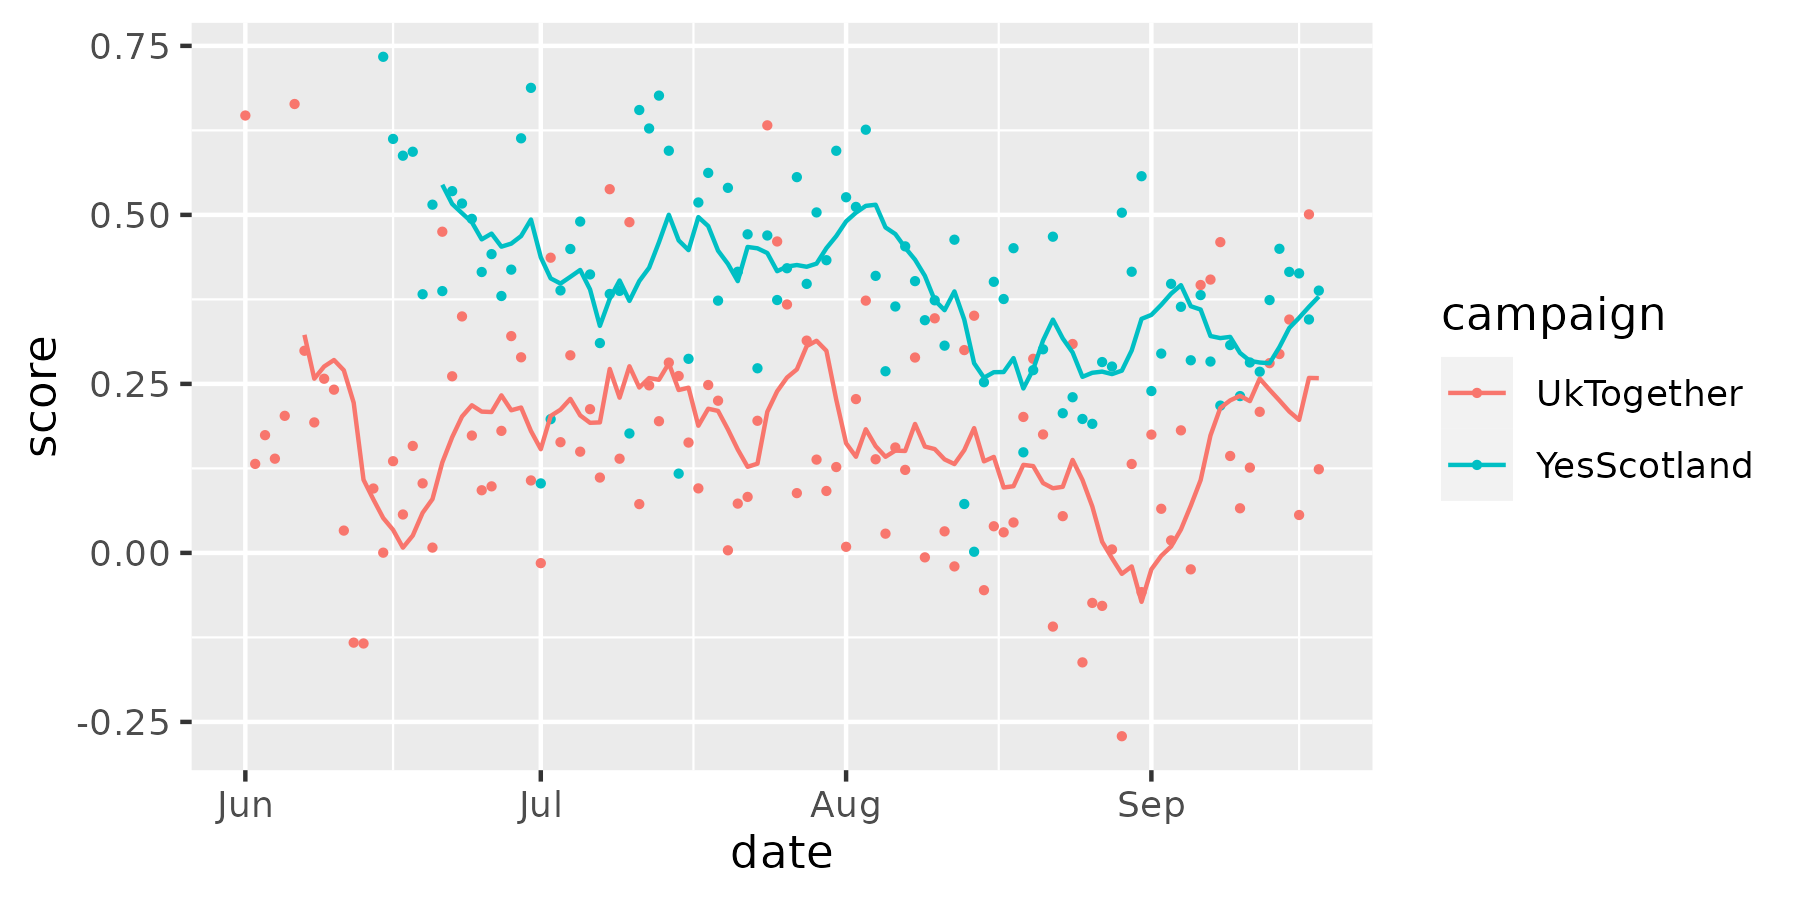
\includegraphics[width=\linewidth]{plots/sentiment_time.png}
\end{figure}

\end{col}

\end{cols}
\end{frame}

\begin{frame}[fragile]{VADER with Python}
\protect\hypertarget{vader-with-python}{}
In python, we can use the
\href{https://github.com/cjhutto/vaderSentiment}{vaderSentiment} package

\medskip
\scriptsize

\begin{Shaded}
\begin{Highlighting}[]
\ImportTok{from}\NormalTok{ vaderSentiment.vaderSentiment }\ImportTok{import}\NormalTok{ SentimentIntensityAnalyzer}

\NormalTok{yes }\OperatorTok{=}\NormalTok{ pd.read\_csv(}\StringTok{"../datasets/YesScotlandTweets\_cleaned.csv"}\NormalTok{)}
\NormalTok{yes[}\StringTok{"campaign"}\NormalTok{] }\OperatorTok{=} \StringTok{"YesScotland"}
\NormalTok{no }\OperatorTok{=}\NormalTok{ pd.read\_csv(}\StringTok{"../datasets/UkTogetherTweets\_cleaned.csv"}\NormalTok{)}
\NormalTok{no[}\StringTok{"campaign"}\NormalTok{] }\OperatorTok{=} \StringTok{"UkTogether"}
\NormalTok{df }\OperatorTok{=}\NormalTok{ pd.concat([yes, no]).reset\_index(drop}\OperatorTok{=}\VariableTok{True}\NormalTok{)}

\NormalTok{analyzer }\OperatorTok{=}\NormalTok{ SentimentIntensityAnalyzer()}

\NormalTok{results }\OperatorTok{=}\NormalTok{ [analyzer.polarity\_scores(x) }\ControlFlowTok{for}\NormalTok{ x }\KeywordTok{in}\NormalTok{ df[}\StringTok{"text"}\NormalTok{]]}
\NormalTok{sentiment }\OperatorTok{=}\NormalTok{ pd.DataFrame.from\_dict(results)}

\NormalTok{sentiment\_df }\OperatorTok{=}\NormalTok{ pd.concat([df,sentiment], axis}\OperatorTok{=}\DecValTok{1}\NormalTok{)}
\NormalTok{sentiment\_df.head()}
\end{Highlighting}
\end{Shaded}

\begin{verbatim}
##    x                                               text  ...    pos  compound
## 0  1  Thank you, everyone! #indyref http://t.co/1kTz...  ...  0.411    0.4199
## 1  2  As the polls close, total likes on the @YesSco...  ...  0.147    0.4754
## 2  3  RT @YESforScotland4: #voteyes YES what a fanta...  ...  0.297    0.8668
## 3  4  We can be proud of #indyref, which has seen a ...  ...  0.147    0.4767
## 4  5  RT @Crafty_Goddess: Txt from 25 year old niece...  ...  0.122    0.4497
## 
## [5 rows x 22 columns]
\end{verbatim}
\end{frame}

\begin{frame}[fragile]{VADER with Python}
\protect\hypertarget{vader-with-python-1}{}
We get the data into the format where there is a row for every day, and
the score for each day is in a column for each campaign

\medskip
\scriptsize

\begin{Shaded}
\begin{Highlighting}[]
\ImportTok{import}\NormalTok{ matplotlib.pyplot }\ImportTok{as}\NormalTok{ plt}
\NormalTok{sentiment\_df[}\StringTok{"date"}\NormalTok{] }\OperatorTok{=}\NormalTok{ pd.to\_datetime(df.created).dt.date}
\NormalTok{daily\_sentiment }\OperatorTok{=}\NormalTok{ (sentiment\_df}
\NormalTok{                   .groupby([}\StringTok{"date"}\NormalTok{,}\StringTok{"campaign"}\NormalTok{])[}\StringTok{"compound"}\NormalTok{]}
\NormalTok{                   .mean()}
\NormalTok{                   .reset\_index()}
\NormalTok{                   .pivot\_table(columns}\OperatorTok{=}\StringTok{"campaign"}\NormalTok{, values}\OperatorTok{=}\StringTok{"compound"}\NormalTok{, index}\OperatorTok{=}\StringTok{"date"}\NormalTok{)}
\NormalTok{                   .reset\_index()}
\NormalTok{                  )}

\NormalTok{daily\_sentiment[}\StringTok{"date"}\NormalTok{] }\OperatorTok{=}\NormalTok{ pd.to\_datetime(daily\_sentiment[}\StringTok{"date"}\NormalTok{])}
\NormalTok{days }\OperatorTok{=}\NormalTok{ pd.date\_range(start}\OperatorTok{=}\StringTok{"2014{-}06{-}01"}\NormalTok{,end}\OperatorTok{=}\StringTok{"2014{-}09{-}18"}\NormalTok{)}
\NormalTok{daily\_sentiment }\OperatorTok{=}\NormalTok{ pd.DataFrame(\{}\StringTok{"date"}\NormalTok{: days\}).merge(daily\_sentiment, how}\OperatorTok{=}\StringTok{"left"}\NormalTok{)}

\NormalTok{daily\_sentiment.head()}
\end{Highlighting}
\end{Shaded}

\begin{verbatim}
##         date  UkTogether  YesScotland
## 0 2014-06-01    0.647000          NaN
## 1 2014-06-02    0.228642          NaN
## 2 2014-06-03    0.174267          NaN
## 3 2014-06-04    0.209287          NaN
## 4 2014-06-05    0.202725          NaN
\end{verbatim}
\end{frame}

\begin{frame}[fragile]{Sentiment over time}
\protect\hypertarget{sentiment-over-time-2}{}
The easiest way to plot this is with base matplotlib

\medskip

\begin{cols}

\begin{col}{0.5\textwidth}

\scriptsize

\begin{Shaded}
\begin{Highlighting}[]
\NormalTok{fig, ax }\OperatorTok{=}\NormalTok{ plt.subplots(figsize}\OperatorTok{=}\NormalTok{(}\DecValTok{6}\NormalTok{,}\DecValTok{4}\NormalTok{))}

\ControlFlowTok{for}\NormalTok{ campaign }\KeywordTok{in}\NormalTok{ [}\StringTok{"UkTogether"}\NormalTok{, }\StringTok{"YesScotland"}\NormalTok{]:}
\NormalTok{    ax.scatter(}
\NormalTok{      daily\_sentiment.date, daily\_sentiment[campaign],}
\NormalTok{      s}\OperatorTok{=}\DecValTok{5}\NormalTok{, alpha}\OperatorTok{=}\FloatTok{0.7}
\NormalTok{    )}
\NormalTok{    x }\OperatorTok{=}\NormalTok{ daily\_sentiment[campaign].rolling(}\DecValTok{7}\NormalTok{).mean()}
\NormalTok{    ax.plot(daily\_sentiment.date, x, label}\OperatorTok{=}\NormalTok{campaign)}

\NormalTok{fig.autofmt\_xdate()}
\NormalTok{ax.legend()}

\NormalTok{plt.savefig(}\StringTok{"plots/sentiment\_time\_py.png"}\NormalTok{)}
\end{Highlighting}
\end{Shaded}

\end{col}

\begin{col}{0.05\textwidth}
~

\end{col}

\begin{col}{0.45\textwidth}

\begin{figure}
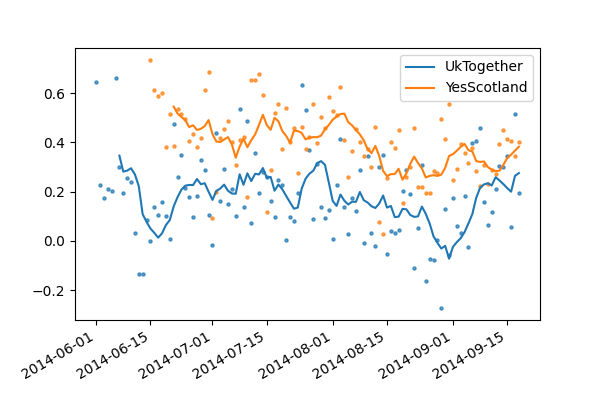
\includegraphics[width=\linewidth]{plots/sentiment_time_py.png}
\end{figure}

\end{col}

\end{cols}
\end{frame}

\begin{frame}{Sentiment analysis in other languages}
\protect\hypertarget{sentiment-analysis-in-other-languages}{}
\begin{itemize}
\tightlist
\item
  \href{https://github.com/KarstenAMF/GerVADER}{GerVADER}
\item
  \href{https://www.cic.ipn.mx/~sidorov/\#SEL}{Spanish Emotion Lexicon}
\end{itemize}
\end{frame}

\hypertarget{fancy-sentiment-analysis}{%
\section{Fancy sentiment analysis}\label{fancy-sentiment-analysis}}

\begin{frame}{Fancy sentiment analysis}
\protect\hypertarget{fancy-sentiment-analysis-1}{}
Fancy NLP does not apply rules that we give it. It \emph{learns} rules
from training data.

Complex models, which encode text in complex ways, have outperformed
lexicon-based sentiment analysis \emph{on the main benchmarked tasks for
which they are often optimized}.

Sentiment datasets are often comprised of movie or product reviews.
\end{frame}

\begin{frame}{Fancy sentiment analysis}
\protect\hypertarget{fancy-sentiment-analysis-2}{}
We will learn more about how training such models work in the next
sessions, but you can access one of many such models
\href{https://huggingface.co/cardiffnlp/twitter-roberta-base-sentiment}{here}.
See also
\href{https://huggingface.co/pysentimiento/robertuito-sentiment-analysis}{Spanish},
\href{https://huggingface.co/oliverguhr/german-sentiment-bert}{German},
\href{https://huggingface.co/turing-usp/FinBertPTBR}{Brazilian
Portuguese},
\href{https://huggingface.co/uer/roberta-base-finetuned-chinanews-chinese}{Chinese}
\end{frame}

\hypertarget{validation}{%
\section{Validation}\label{validation}}

\begin{frame}{Validation}
\protect\hypertarget{validation-1}{}
Almost all methods for sentiment analysis are validated, but almost none
are validated on your dataset. Unless your dataset is very similar to
the validation dataset, you should validate yourself.

This means selecting a random sample of your texts, labelling the
sentiment of these texts by hand, then comparing the label you gave with
the score given by your method.

If your method gives the same label as you in 100\% of cases, then you
have an accuracy of 100\%.

We will explore validation metrics in the next session on supervised
learning.
\end{frame}

\begin{frame}{Exercise - validating on your own data}
\protect\hypertarget{exercise---validating-on-your-own-data}{}
\begin{itemize}
\tightlist
\item
  In a spreadsheet, write 5 texts that express your feelings about
  recent political events, with each text in a new row of the same
  column
\item
  Ask your neighbour to rate the sentiment of your texts in the
  neighbouring column. The value should be between -1 (completely
  negative) and 1 (completely positive).
\item
  Apply one of the techniques we have learnt today to your texts and
  compare with the human annotation
\item
  What is the average (absolute) difference between your human label and
  the automated technique?
\item
  For what text is the divergence greatest?
\end{itemize}
\end{frame}

\hypertarget{examples-in-research}{%
\section{Examples in research}\label{examples-in-research}}

\begin{frame}{Tones from a Narrowing Race}
\protect\hypertarget{tones-from-a-narrowing-race}{}
In
\href{https://www.cambridge.org/core/journals/british-journal-of-political-science/article/tones-from-a-narrowing-race-polling-and-online-political-communication-during-the-2014-scottish-referendum-campaign/49CEE09374F4729B4C0B7048FBA4521C}{Tones
from a Narrowing Race: Polling and Online Political Communication during
the 2014 Scottish Referendum Campaign}, Evelyne Brie and Yannick
Dufresne set out to investigate the dynamics of how political campaigns
use negative communication.

They use the data that we've just seen: tweets sent by the
pro-independence and pro-union campaigns in the Scottish independence
referendum of 2014.
\end{frame}

\begin{frame}{Tones from a Narrowing Race: Obectives}
\protect\hypertarget{tones-from-a-narrowing-race-obectives}{}
The authors want to provide evidence on negative campaigning \emph{in
practice} that complements political theory about how and why actors use
negative campaigning.

They are interested in how real organisations use twitter, meaning their
findings are not subject to the same external validity concerns
generated by the unrepresentativeness of twitter.
\end{frame}

\begin{frame}[fragile]{Tones from a Narrowing Race: Results}
\protect\hypertarget{tones-from-a-narrowing-race-results}{}
\begin{cols}

\begin{col}{0.5\textwidth}
The authors' analysis, which uses the Opinion Observer lexicon (I think
available with the ``bing'' option in tidytext's
\texttt{get\_sentiments()}) finds a similar pattern of sentiment scores
in the different campaigns over time

\end{col}

\begin{col}{0.05\textwidth}
~

\end{col}

\begin{col}{0.45\textwidth}

\begin{figure}
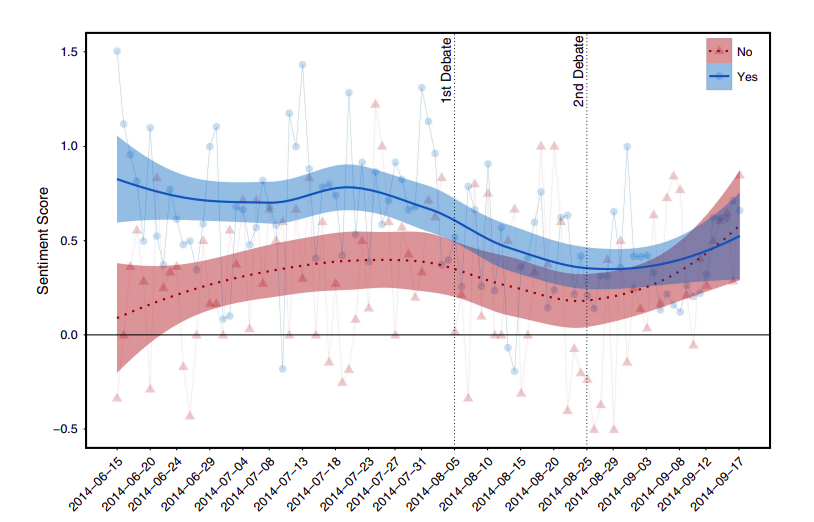
\includegraphics[width=\linewidth]{images/narrowing-fig3.png}
\end{figure}

\end{col}

\end{cols}
\end{frame}

\begin{frame}{Tones from a Narrowing Race: Results}
\protect\hypertarget{tones-from-a-narrowing-race-results-1}{}
\begin{cols}

\begin{col}{0.5\textwidth}
They find a significant relationship between the no campaign leading in
the polls and the negativity of their tweets. The more NO leads, the
more negatively they tweet.

\medskip

In a simpler model, there is a significant relationship between the
number of days to the election and the negativity of the YES campaign.
That is, the decline in positivity as the election is statistically
significant.

\medskip

There is also evidence that the YES campaign tweeted more negatively the
day after each debate (which they were said to have lost)

\end{col}

\begin{col}{0.05\textwidth}
~

\end{col}

\begin{col}{0.45\textwidth}

\begin{figure}
\only<1>{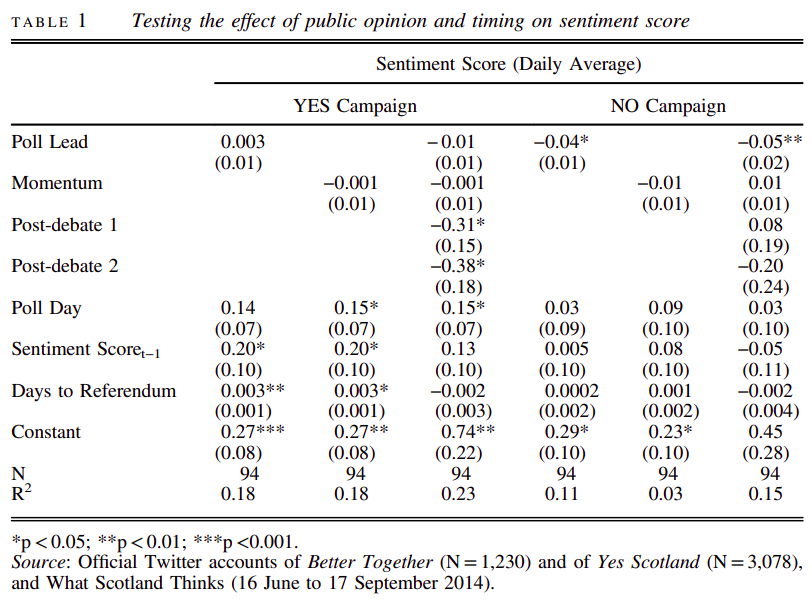
\includegraphics[width=\linewidth]{images/narrowing-table1.png}}
\only<2>{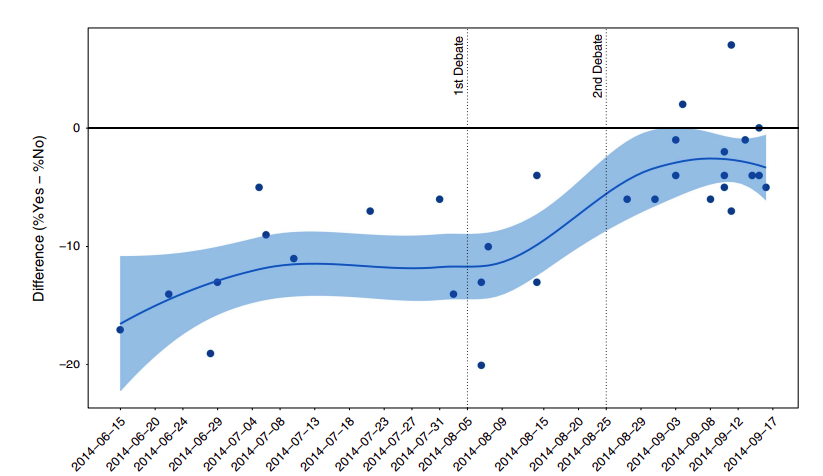
\includegraphics[width=\linewidth]{images/narrowing-fig1.png}}
\end{figure}

\end{col}

\end{cols}
\end{frame}

\begin{frame}{Discusion}
\protect\hypertarget{discusion}{}
What does this tell us about the scottish election campagin?

What does this tell us about negative communication in political
campaigns in general?

What potential confounding factors might explain the results?
\end{frame}

\begin{frame}{Other examples}
\protect\hypertarget{other-examples}{}
\begin{itemize}
\tightlist
\item
  \href{https://journals.plos.org/plosone/article?id=10.1371/journal.pone.0195750}{Baylis
  and Obradovich et al.} explore how weather affects sentiment
\item
  \href{https://www.cambridge.org/core/journals/european-political-science-review/article/abs/going-in-circles-the-influence-of-the-electoral-cycle-on-the-party-behaviour-in-parliament/B4693B1A27049DB3BCE314F32D6BD1EB}{Schwalbach}
  looks at how political debate varies in sentiment through the
  legislative period, depending on their involvement in the government.
\item
  \href{https://www.nature.com/articles/s41562-022-01312-y}{Wang et al.}
  explore how the COVID-19 pandemic affected how people expressed
  sentiment
\item
  \href{https://link.springer.com/chapter/10.1007/978-3-030-66891-4_9}{Arratia
  et al.} describe how sentiment analysis is used to provide information
  about financial markets
\end{itemize}
\end{frame}

\hypertarget{wrapup-and-outlook}{%
\section{Wrapup and Outlook}\label{wrapup-and-outlook}}

\begin{frame}{Wrapup}
\protect\hypertarget{wrapup}{}
So far in this course, we have covered:

\begin{itemize}
\tightlist
\item
  How to get texts from tricky places
\item
  How to process them and manipulate them
\item
  How to represent them in different ways
\item
  How to find the similarity between texts
\item
  Hot to find what texts are about
\end{itemize}

Now we know how to find out what emotions are present in texts
\end{frame}

\begin{frame}{Outlook}
\protect\hypertarget{outlook}{}
We said sentiment analysis is a special case of classification. We will
explore this in detail next week when we cover \textbf{supervised text
classification}.

We'll be training machine learning classifiers to assign documents to
predefined classes, and learning how to evaluate how well these work.

This is the last major technique we will learn, before the penultimate
session where we will find about how to apply a range of the techniques
we have seen using the fanciest most up-to-date methods.
\end{frame}

\begin{frame}{Homework assignment (optional)}
\protect\hypertarget{homework-assignment-optional}{}
Take a protocol from the Bundestag and process it as you did in
Assignment 1

Using a German sentiment lexicon, calculate a sentiment score for each
speech.

Show the average sentiment score for each party.

Show the 5 speeches with the most positive sentiment, and the 5 speeches
with the most negative sentiment.
\end{frame}

\begin{frame}[allowframebreaks]{}
  \bibliographytrue
  \bibliography{../presentation-resources/MyLibrary.bib}
\end{frame}

\end{document}
